%% DIW-GC LaTeX Beamer presentation template (requires beamer package)
%% This Template is still evolving - it might differ in future releases!

\documentclass{beamer}

\mode<presentation>


%%%%%%%%%%%%%%%%%%%%%%%%%%%%%%%%%%%%%%%%%%%%
\usetheme{diwgc}   
% Options:
%no option = no footline
%[showfootline=true] = show footline with [shortname], [shorttitle] and GC-Logo
%[showframenumbers=true] = show footline with [shortname], [shorttitle], framenumbers and GC-Logo
%[showlogo=true] = show empty footline but with GC-Logo
%[showlogoonly=true] = show the GC-Logo only

%% These are the outer themes. Try them and choose the one you like.
%% NOTE: The option "[subsection=false]" is only available in the "smoothbars" outer theme.

%\useoutertheme[subsection=false]{smoothbars}
%\useoutertheme[subsection=true]{smoothbars}
%\useoutertheme{shadowdiwgc}
%\useoutertheme{splitdiwgc}
%\useoutertheme{shadow}




%% Add packages here
\usepackage{graphicx}





\title[Your shorttitle]{This is the title of your presentation}
\subtitle{This is the subtitle of your presentation}
\author[Your shortname]{Your name goes here}
\institute{DIW Berlin Graduate Center}
\date{\today} 
%\date{September 28, 2012}


\begin{document}


\begin{frame}[plain] 
\titlepage
\end{frame}



\begin{frame}
\frametitle{Outline}
\tableofcontents 
\end{frame}

 
\section{Introduction}
\subsection{Subsection 1}
\begin{frame} 
\frametitle{This is the Introduction}
\framesubtitle{Subtitles are not really necessary (and don't look good)}
\begin{itemize}
  \item Item One \newline
  \item Item Two \newline
  \item Item Three \newline
  \item Item Four \newline
  \item Item Five \newline
  \item Item Six
\end{itemize}
\end{frame}



\subsection{Subsection 2}
\begin{frame}
\frametitle{Enumeration}
  \begin{enumerate}
    \item First item. \newline
    \item Second item. \newline 
    \item Third item. \newline
    \item Fourth item. \newline
    \item Fifth item. \newline 
    \item Sixth item. \newline
  \end{enumerate}
\end{frame} 


\subsection{Subsection 3}
\begin{frame}
\frametitle{Here some boxes}
\begin{block}{Blocktitel}
        Blocktext
\end{block}

Beispielblock

\begin{exampleblock}{Beispielblocktitel}
        \begin{equation} \frac{4}{3}\pi rˆ2 \end{equation}
\end{exampleblock}


Warnungsblock

\begin{alertblock}{Warnungsblocktitel}
        Warnungsblocktext
\end{alertblock}
\end{frame}



%% In case you need full space of a slide for pictures and diagrams use the option [plain].
\begin{frame}[plain]
\begin{figure}
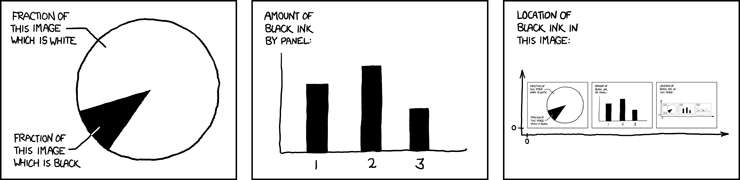
\includegraphics[height=8.5cm]{self_description.png}
\caption{http://xkcd.com/688/}
\end{figure}
\end{frame}



%% If you do not want to use a last page just uncomment these lines or delete them.

%%%%%%%%%%%%%%%%%%%%%%%%%%%%%%%%% Last Page %%%%%%%%%%%%%%%%%%%%%%%%%%%%%%%%%%%%%%%%%%%%%%%%%%%%%%%

 
\newcommand{\LastPageText}{Your text goes right here!}
\begin{frame}[plain]
\lastpage
\end{frame}


%%%%%%%%%%%%%%%%%%%%%%%%%%%%%%%%%%%%%%%%%%%%%%%%%%%%%%%%%%%%%%%%%%%%%%%%%%%%%%%%%%%%%%%%%%%%%%%%%%%

\mode
<all>


\end{document}

